\chapter{입자역학에서 고전장으로}

\section{장이란 무엇인가}

앞선 강의에서는 불변 작용에서 출발해 상대론적 입자역학을 전개했다. 이제 역학의 대상을 바꾸어 고전장론을 다룬다. 양자장론이 아니다. 양자역학은 때때로 유용한 비교 대상이 되지만, 이 장의 방정식은 보통의 고전장을 기술한다. 배경에는 익숙한 모형인 전자기학이 있다. 전자기파는 공간을 전파하며 하전 입자와 상호작용한다. 먼저 더 간단한 장부터 살펴보자.

시공간에는 여러 공간 좌표가 있을 수 있지만 시간 좌표는 하나다. 다음과 같이 쓰자.
\begin{equation}
x^\mu=(t,x^1,\ldots,x^d),
\end{equation}
여기서 공간 첨자는 \(i=1,\ldots,d\)이다. \(d\)의 값은 우리 세계처럼 3일 수도 있고, 모형에 따라 1, 2, 9, 25 또는 그 밖의 어떤 수일 수도 있다. 여기서 중요한 비대칭성은 여전히 시간 방향이 하나뿐이라는 점이다. 이 강의에서는 시간이 여러 개인 이론이 왜 그렇게 어려운지 설명하려 하지 않는다. 그저 보통의 인과적 물리학이 정식화되는 시간 하나의 틀을 채택한다.

장은 공간과 시간에 따라 값이 달라질 수 있는 관측 가능한 물리량이다. 간단한 예로 온도를 들 수 있다.
\begin{equation}
T=T(\mathbf{x},t).
\end{equation}
온도는 각 사건에 하나의 수를 대응시키므로 스칼라장이다. 풍속도 공간과 시간에 따라 변하지만, 크기와 방향을 가지므로 여러 성분으로 이루어진 벡터장이다. 상대론적 물리학에서 자연스러운 벡터는 세 성분이 아니라 네 성분을 갖는다.

이 강의의 대부분에서는 성분이 하나인 장을 \(f\)에 해당하는 그리스 문자로 나타낸다.
\begin{equation}
\phi=\phi(\mathbf{x},t).
\label{eq:sr4-field-definition}
\end{equation}
\(\phi\)를 스칼라라고 부르는 것은 결국 단순히 성분이 하나라는 뜻을 넘어선다. 같은 물리적 사건에 대해 모든 관성 관측자가 \(\phi\)에 같은 값을 부여한다는 뜻이다. 이 변환 법칙은 변분 역학을 세운 뒤에 도입한다.

\section{입자의 기본 모형}

\subsection{\texorpdfstring{\(\phi\)}{파}}

장론으로 가는 가장 빠른 길은 잠시 물러나 보통의 비상대론적 입자를 살펴보는 것이다. 입자가 직선 위를 움직인다고 하고, 그 좌표를 \(\phi\) 대신 \(x\)라고 부르자. 좌표를 반드시 \(x\)라고 이름 붙여야 할 수학적 이유는 없다. 다가올 유사성을 드러내기 위해 이례적인 이름을 택한 것이다. 시간을 가로축으로 그리면 입자의 전체 이력은 \(\phi(t)\)라는 곡선이 되며, 양수와 음수 값을 모두 지날 수 있다.

초기 시각과 최종 시각 \(a\) 및 \(b\)를 고정하면 작용은 다음과 같다.
\begin{align}
A[\phi]
&=\int_a^b dt\,L(\phi,\dot\phi),\\
L(\phi,\dot\phi)
&=\frac{m}{2}\dot\phi^{\,2}-V(\phi).
\label{eq:sr4-particle-lagrangian}
\end{align}
오일러--라그랑주 방정식은 다음과 같다.
\begin{equation}
\frac{d}{dt}\left(\frac{\partial L}{\partial\dot\phi}\right)
-\frac{\partial L}{\partial\phi}=0.
\label{eq:sr4-particle-el}
\end{equation}
\eqref{eq:sr4-particle-lagrangian}의 라그랑지언에 대해서는
\begin{equation}
\frac{\partial L}{\partial\dot\phi}=m\dot\phi,
\qquad
\frac{\partial L}{\partial\phi}=-\frac{dV}{d\phi},
\end{equation}
이므로
\begin{equation}
\boxed{m\ddot\phi=-\frac{dV}{d\phi}}.
\label{eq:sr4-newton}
\end{equation}
이는 좌표를 \(\phi\)로 써서 나타낸 뉴턴 방정식일 뿐이다.

\begin{figure}[htbp]
\centering
\includegraphics[width=0.90\textwidth]{lecture_04_figure_01.png}
\caption{좌표 \(\phi(t)\)에 대한 보통의 오일러--라그랑주 방정식과 그 뉴턴 역학적 결과.}
\lectureframe{00:10:18}
\end{figure}

물리적 경로는 양 끝점을 고정했을 때 작용을 정지값으로 만든다. 강의에서는 흔히 \emph{최솟값}이라고 하지만, 정확한 표현은 정지성이다. 경로는 최솟값이나 최댓값 또는 다른 정지값을 줄 수 있다. 유용한 직관적 모형으로 시간 구간을 작은 조각 여러 개로 나누어 보자. 그러면 작용은 표본화한 여러 \(\phi\)값의 함수가 된다. 양 끝점은 그대로 둔 채 이 값들을 바꾸고 각각에 대해 미분하는 것이 오일러--라그랑주 방정식의 유한 차원적 선구 형태다.

\subsection{\texorpdfstring{\(0+1\)}{01}차원에서의 역학}

이제 공간 차원은 없고 시간만 있는 세계를 상상해 보자. 그 세계의 공간은 한 점이다. 의존할 위치가 없으므로 그 세계의 장은 위치에 의존할 수 없으며, 오직 \(\phi(t)\)라는 함수일 수 있다. 따라서 좌표 하나를 갖는 보통의 입자역학을 \(0+1\)차원의 장론으로 읽을 수 있다. 수학은 달라지지 않았다. 입자의 위치라는 해석이 공간 없는 세계에서 장의 값이라는 해석으로 바뀌었을 뿐이다.

\begin{figure}[htbp]
\centering
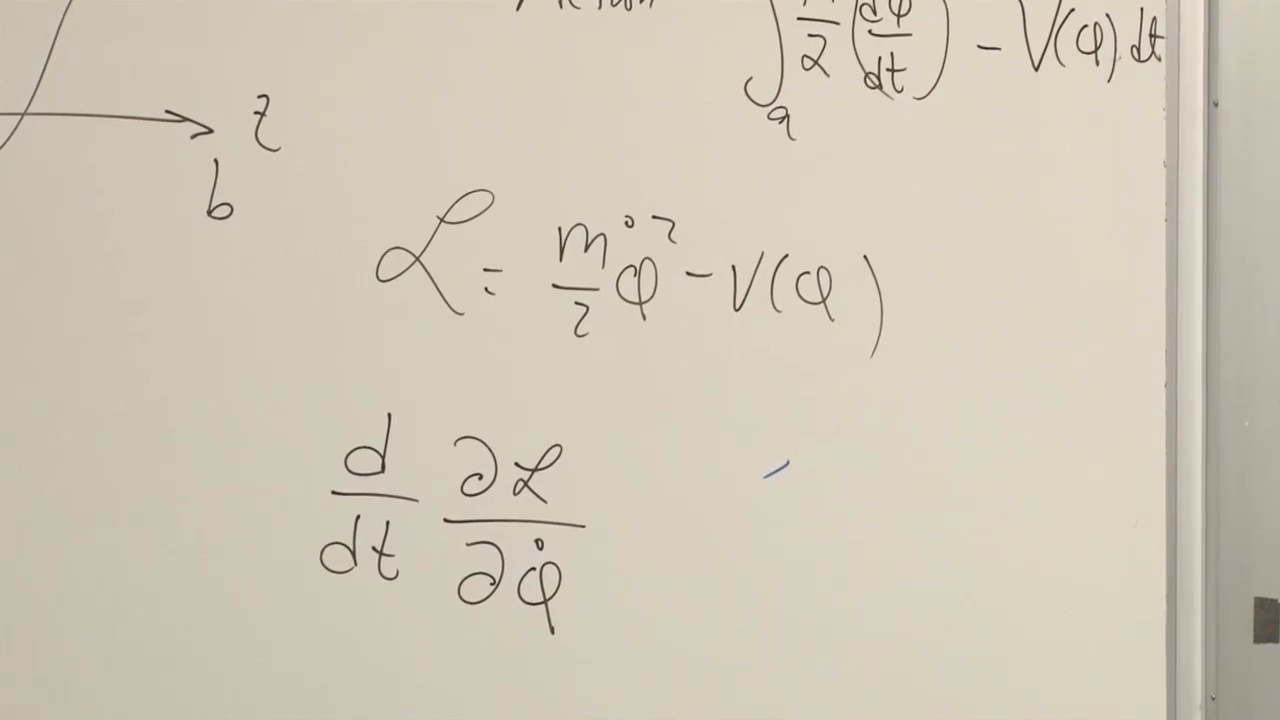
\includegraphics[width=0.90\textwidth]{lecture_04_figure_02.png}
\caption{표본화한 이력 \(\phi(t)\): 입자의 궤적이자, 새롭게 해석하면 \(0+1\)차원에서 장의 이력.}
\lectureframe{00:14:30}
\end{figure}

\begin{classroomqa}
\audiencequestion{공간 차원이 없으면 퍼텐셜은 사라지나요?}
\lecturerresponse{아닙니다. 공간적 변화는 사라져도 장에는 여전히 값이 있습니다. 에너지는 \(V(\phi)\)를 통해 그 값에 의존할 수 있습니다. 입자로 해석하면 곡선을 위아래로 옮길 때 퍼텐셜 에너지가 달라지고, 장으로 해석하면 서로 다른 \(\phi\) 값이 서로 다른 퍼텐셜 에너지를 갖습니다. \lecturetimestamp{00:15:00}}
\end{classroomqa}

\begin{classroomqa}
\audiencequestion{공간이 전혀 없는 경우 대신, 장이 시간에만 의존하는 보통의 공간을 상상해도 되나요?}
\lecturerresponse{네. 이 목적에서는 국소적인 수학이 같습니다. 모든 공간 미분이 사라지고 \(\phi(t)\)만 남습니다. 이를 \(0+1\)차원 이론이라고 부르면 축소된 구조를 분리해 볼 수 있지만, 더 큰 세계에서 공간적으로 균일한 장을 떠올려도 같은 직관을 얻을 수 있습니다. \lecturetimestamp{00:16:25}}
\end{classroomqa}

이 우회 과정의 요점이 이제 분명해졌다. 한 좌표인 시간에 의존하는 장에 대한 작용 원리를 알고 있다. 이 원리의 형태를 이용해 시공간의 모든 좌표에 의존하는 장의 작용 원리를 추측할 수 있다.

\section{시공간에 펼쳐진 장의 이력}

\subsection{곡선에서 곡면으로}

\(1+1\)차원에서 시공간 자체는 \(t\)와 \(x\)을 좌표로 하는 평면이다. 장의 값 \(\phi(x,t)\)은 세 번째 방향을 이룬다. 따라서 장의 이력은 곡선이 아니라 시공간 평면 위에 놓인 곡면이다. 스칼라장은 양수일 필요가 없으므로 곡면은 0보다 위로 솟거나 아래로 내려갈 수 있다.

\begin{figure}[htbp]
\centering
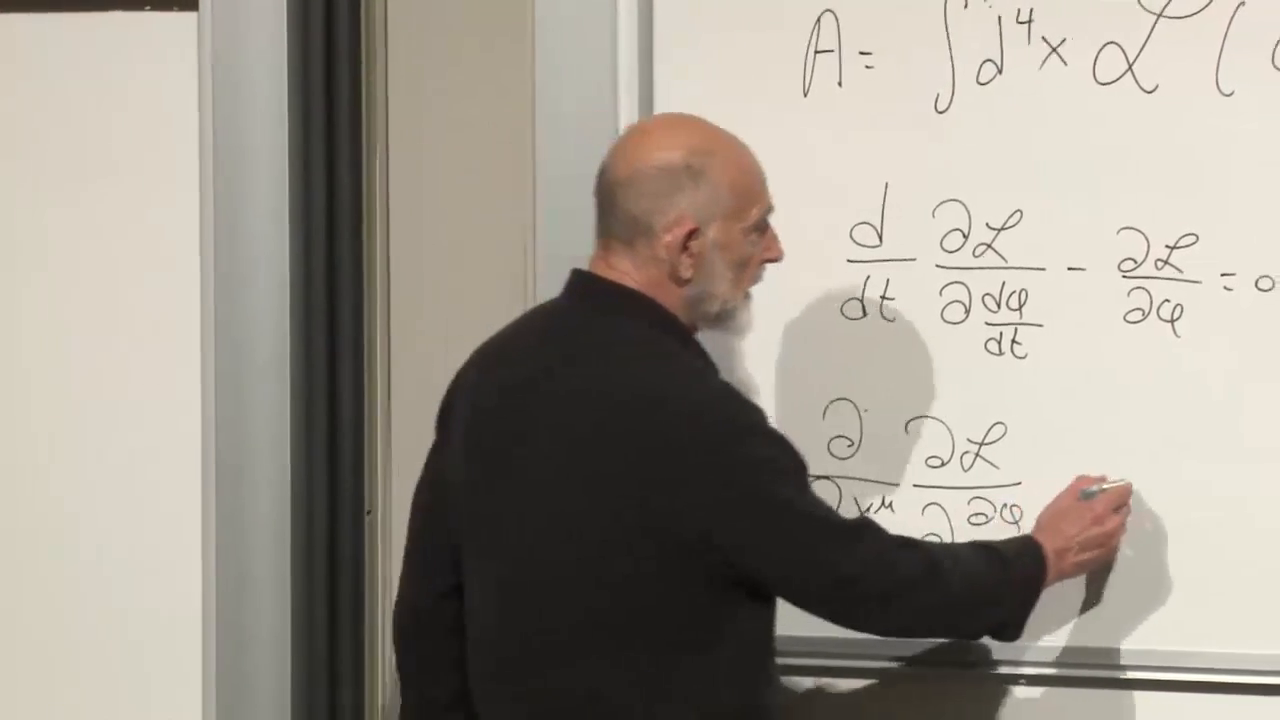
\includegraphics[width=0.90\textwidth]{lecture_04_figure_03.png}
\caption{\(1+1\)차원 시공간 평면 위의 곡면으로 나타낸 스칼라장의 이력.}
\lectureframe{00:20:46}
\end{figure}

우리의 물리적 시공간은 공간 3차원과 시간 1차원으로 이루어진 \(3+1\)차원 시공간이라고 부른다. 탁자 위의 모형은 \(2+1\)차원이고, 철사에 구슬을 꿰어 놓은 모습은 \(1+1\)차원의 세계를 떠올리게 한다. \(\phi\)을 그리려면 축 하나가 더 필요하므로 \(3+1\) 경우조차 충실하게 그릴 수는 없다. 하지만 정의는 명확하다. 완전한 이력은 모든 시공간 사건에 \(\phi\)의 값 하나를 대응시킨다.

\subsection{고정된 양 끝점에서 고정된 경계 자료로}

입자의 변분 문제에서는 양 끝점을 고정하고 그 사이의 곡선을 변분한다. 이에 대응하는 장론의 문제에서는 시공간 영역을 정하고 그 경계에서 \(\phi\)를 고정한 뒤 내부의 \(\phi\)를 변분한다. 그 영역은 \(1+1\)차원 그림의 직사각형일 수도 있고, 더 높은 차원의 시공간에 있는 적절한 임의의 영역일 수도 있다.

\begin{figure}[htbp]
\centering
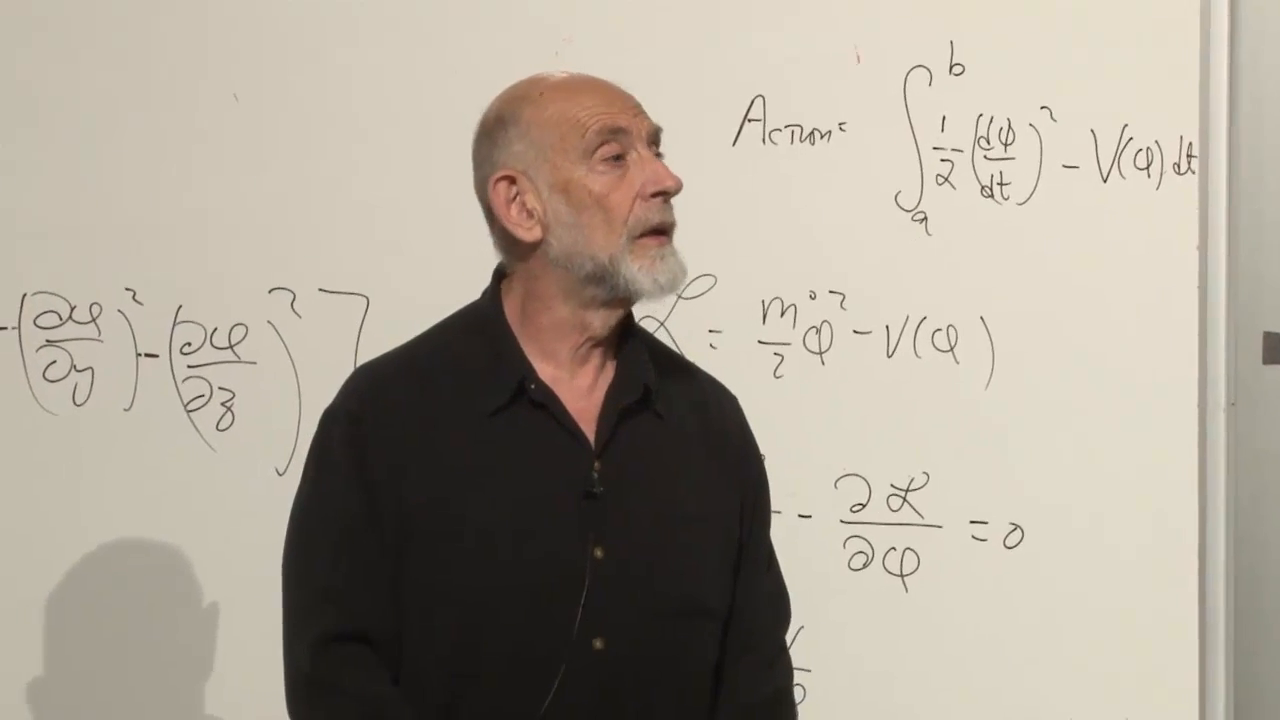
\includegraphics[width=0.90\textwidth]{lecture_04_figure_04.png}
\caption{시공간 영역의 경계 전체를 고정한 채 내부의 장을 변분한다.}
\lectureframe{00:24:52}
\end{figure}

\begin{classroomqa}
\audiencequestion{퍼텐셜이 시간에 명시적으로 의존해도 라그랑지언 정식화가 유효한가요?}
\lecturerresponse{네. 오일러--라그랑주 정식화와 해밀턴 정식화는 여전히 유효합니다. 일반적으로 사라지는 것은 에너지 보존입니다. 시간에 대한 명시적 의존성은 시간 병진 대칭성을 깨뜨립니다. 장론에서도 시공간에 대한 명시적 의존성을 허용할 수 있지만, 그에 따른 보존 법칙에 영향을 줍니다. \lecturetimestamp{00:23:49}}
\end{classroomqa}

\begin{classroomqa}
\audiencequestion{직사각형 모양의 장 영역에서는 위쪽과 아래쪽만 고정하나요, 아니면 경계 전체를 고정하나요?}
\lecturerresponse{이 변분 구성에서는 경계 전체를 고정합니다. \(1+1\)차원 직사각형의 네 변 모두를 고정합니다. 장은 내부에서만 요동할 수 있습니다. 이는 입자역학에서 양 끝점을 모두 고정하는 것에 직접 대응합니다. \lecturetimestamp{00:24:24}}
\end{classroomqa}

경계 전체를 고정한다는 것은 방정식을 유도할 때 사용하는 변분에 관한 설명이다. 이렇게 얻은 쌍곡형 장 방정식을 물리적 시간 진화 문제로 다룰 때는 적절한 초기 자료를 지정하고 방정식이 이를 미래로 전파하도록 두는 것이 더 일반적이다.

\section{작용과 장의 오일러--라그랑주 방정식}

\subsection{라그랑지언 밀도}

시공간 영역을 작은 셀들로 나누자. 작용은 각 셀의 국소적 기여를 모두 더한 값이라고 가정한다. 연속체 극한에서 그 합은 시공간 적분이 된다.
\begin{equation}
A[\phi]
=
\int_{\Omega} d^4x\,
\mathcal{L}\!\left(
\phi,\partial_\mu\phi;x^\mu
\right),
\qquad
d^4x=dt\,dx\,dy\,dz.
\label{eq:sr4-field-action}
\end{equation}
\(\mathcal{L}\)는 라그랑지언 밀도다. \(\mathcal{L}(\phi,\partial_\mu\phi;x^\mu)\)의 세미콜론은 역학적 논변과 좌표에 대한 명시적 의존 가능성을 구분한다. 균일한 폐쇄계에서는 보통 후자의 의존성이 없지만, 변분 형식은 이를 금하지 않는다.

간결한 표기
\begin{equation}
\partial_\mu\phi
\equiv
\frac{\partial\phi}{\partial x^\mu}
\end{equation}
는 시간 미분과 공간 미분을 한데 나타낸다. 강의의 성분 표기법으로는 다음과 같이 쓸 수도 있다.
\begin{equation}
\begin{aligned}
\phi_t&=\frac{\partial\phi}{\partial t},\\
\phi_x&=\frac{\partial\phi}{\partial x},\\
\phi_y&=\frac{\partial\phi}{\partial y},\\
\phi_z&=\frac{\partial\phi}{\partial z}.
\end{aligned}
\label{eq:sr4-component-derivatives}
\end{equation}
입자가 여러 좌표를 가질 수 있듯 장도 여러 개일 수 있다. 지금은 장이 \(\phi\) 하나뿐이다.

\(d^4x\)는 네 좌표에 대한 측도를 간략하게 쓴 기호일 뿐이다. 다른 차원의 시공간에서는 이를 \(d^Dx\)로 바꾸어야 한다. \(0+1\)차원 기본 모형에서는 \(D=1\)이고 \(d^1x\)는 그저 \(dt\)이다.

\begin{figure}[htbp]
\centering
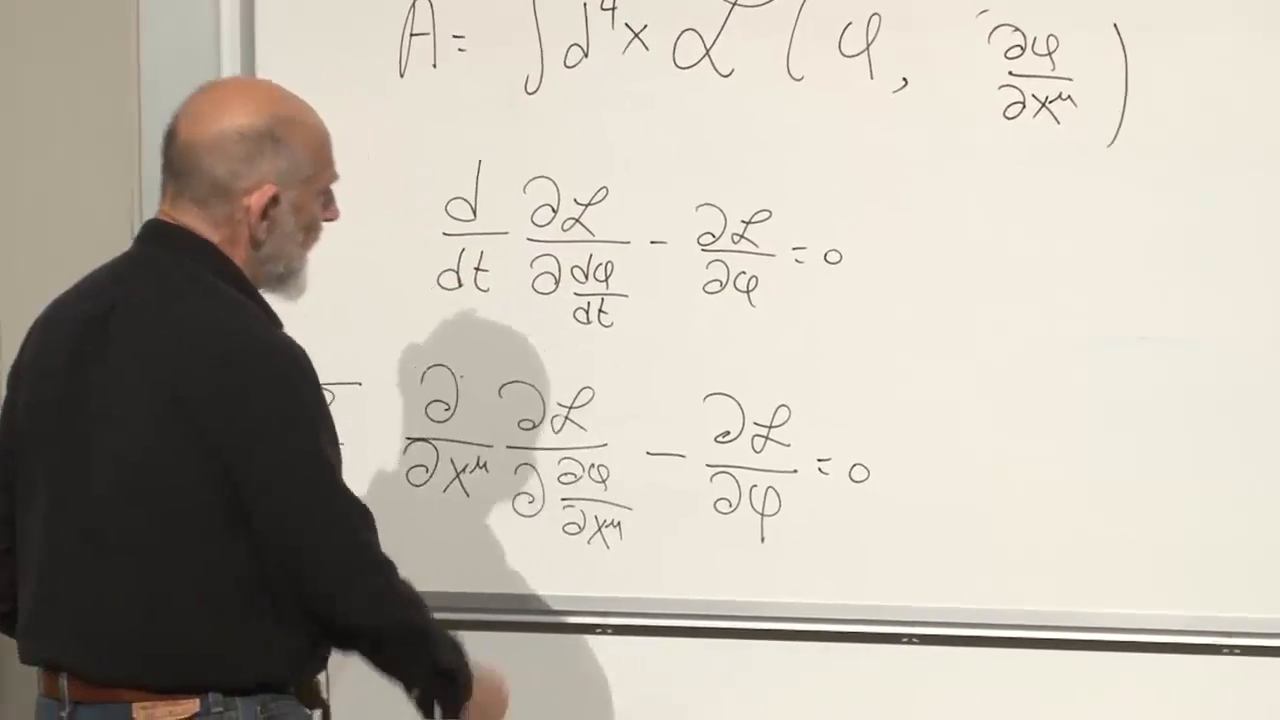
\includegraphics[width=0.90\textwidth]{lecture_04_figure_05.png}
\caption{국소 함수로 쓴 작용 밀도: \(\phi\)와 그 시공간 미분에 의존한다.}
\lectureframe{00:32:51}
\end{figure}

\begin{classroomqa}
\audiencequestion{라그랑지언 밀도도 \(x,y,z\) 자체에 의존할 수 있나요?}
\lecturerresponse{가능합니다. 입자 라그랑지언이 \(t\)에 명시적으로 의존할 수 있는 것과 같습니다. 병진 대칭인 폐쇄계에서는 보통 그렇지 않지만, 좌표에 명시적으로 의존해도 형식 자체는 유효합니다. \lecturetimestamp{00:30:29}}
\end{classroomqa}

\begin{classroomqa}
\audiencequestion{지금까지의 구성은 스칼라장에만 해당하나요, 아니면 일반적인가요?}
\lecturerresponse{지금까지의 변분 구조는 일반적입니다. 성분을 하나만 쓴 것은 스칼라장을 암시합니다. 벡터장이나 여러 장의 모음에는 성분 표지가 더 붙고, 각 성분을 모두 변분해야 합니다. \lecturetimestamp{00:31:00}}
\end{classroomqa}

\subsection{격자 모형}

촘촘한 시공간 격자에서는 미분이 이웃한 장 값 사이의 유한 차분이 된다. 그러면 작용은 여러 변수의 보통 함수가 된다. 한 방향에 점이 10개, 다른 방향에 점이 8개인 격자만으로도 장 변수는 이미 80개다. 격자를 세분할수록 변수의 수는 늘어나지만, 최소화 규칙은 여전히 간단하다. 내부의 각 점에서 장의 값에 대해 작용을 미분하고 그 결과를 0으로 둔다.

\begin{figure}[htbp]
\centering
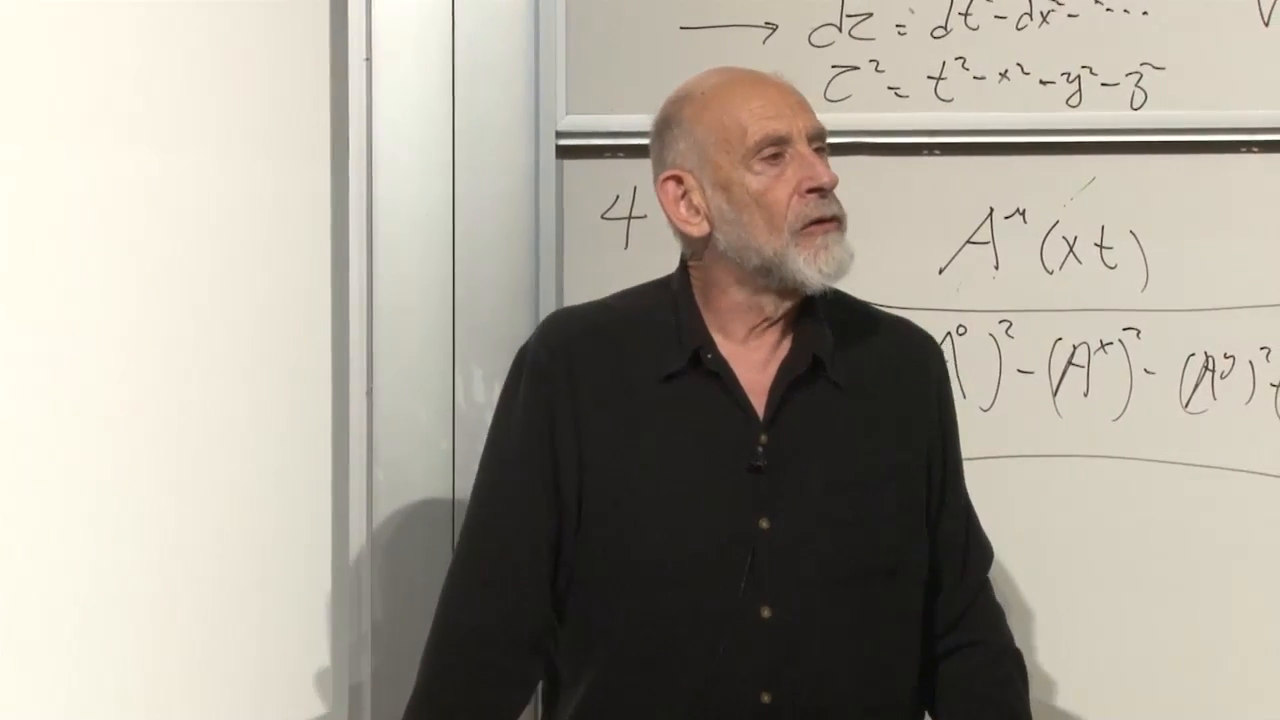
\includegraphics[width=0.90\textwidth]{lecture_04_figure_06.png}
\caption{시공간 영역을 셀들로 나누어, 연속체 극한을 취하기 전에 작용이 여러 변수의 보통 함수가 되도록 한 모습.}
\lectureframe{00:34:05}
\end{figure}

연속체 극한을 취하면 장의 오일러--라그랑주 방정식이 된다.
\begin{equation}
\boxed{
\partial_\mu
\left[
\frac{\partial\mathcal{L}}
{\partial(\partial_\mu\phi)}
\right]
-
\frac{\partial\mathcal{L}}{\partial\phi}
=0
}.
\label{eq:sr4-field-el}
\end{equation}
반복된 \(\mu\)는 모든 시공간 방향에 대해 합산한다. 합산 약식 없이 쓰면 같은 방정식은 다음과 같다.
\begin{align}
&
\frac{\partial}{\partial t}
\left(\frac{\partial\mathcal{L}}{\partial\phi_t}\right)
+
\frac{\partial}{\partial x}
\left(\frac{\partial\mathcal{L}}{\partial\phi_x}\right)
+
\frac{\partial}{\partial y}
\left(\frac{\partial\mathcal{L}}{\partial\phi_y}\right)
\nonumber\\
&\hspace{3em}
+
\frac{\partial}{\partial z}
\left(\frac{\partial\mathcal{L}}{\partial\phi_z}\right)
-
\frac{\partial\mathcal{L}}{\partial\phi}
=0.
\label{eq:sr4-field-el-expanded}
\end{align}
첫째 항은 익숙한 입자역학의 항이다. 장론에서는 각 공간 방향마다 이에 대응하는 항이 하나씩 추가된다. 마지막 항 \(-\partial\mathcal{L}/\partial\phi\)는 바뀌지 않는다.

\begin{figure}[htbp]
\centering
\includegraphics[width=0.90\textwidth]{lecture_04_figure_07.png}
\caption{1차원 오일러--라그랑주 방정식과 그 시공간 일반화를 위아래로 나란히 썼다.}
\lectureframe{00:38:44}
\end{figure}

이 분야는 연속체 역학이라고도 불린다. 자유도에 따라 같은 수학으로 유체 흐름, 탄성 변위 또는 다른 연속 매질을 기술할 수 있다.

\begin{classroomqa}
\audiencequestion{시간은 없고 공간만 있는 세계에서도 같은 방정식이 성립하나요?}
\lecturerresponse{네, 순수한 공간적 변분 문제로는 성립합니다. 물리적으로는 정적 해를 구할 때 이렇게 합니다. 장이 시간에 의존하지 않는다고 가정하고 시간 미분을 모두 버린 뒤 남은 공간 방정식을 풉니다. 시간에 따라 변하지 않는 전기장이나 자기장 구성이 그 예입니다. \lecturetimestamp{00:40:05}}
\end{classroomqa}

\section{가장 단순한 스칼라장 동역학 추측하기}

\subsection{부호가 모두 같을 수 없는 이유}

입자의 운동에너지 항 \(\tfrac12\dot\phi^2\)로 돌아가고, 중요하지 않은 전체 계수는 1로 두어 이를 일반화해 보자. 첫 추측은 다음과 같을 수 있다.
\begin{equation}
\mathcal{L}_{+}
=
\frac12
\left[
\phi_t^2+\phi_x^2+\phi_y^2+\phi_z^2
\right].
\label{eq:sr4-all-plus}
\end{equation}
이는 유용한 오답이다. 시간과 공간에 같은 부호를 부여하기 때문이다. 그 결과 얻는 방정식에는 파동 전파의 쌍곡형 구조가 나타나지 않는다. 올바른 상대론적 조합에서는 시간의 부호와 공간의 부호가 서로 반대다.

\begin{classroomqa}
\audiencequestion{모든 항의 부호가 같은 식이 틀린 것은 라그랑지언이 상대론적 불변량이어야 하기 때문인가요?}
\lecturerresponse{그것이 더 근본적인 답이며 옳습니다. 강의에서는 먼저 더 기초적인 방식으로 부호에 도달합니다. 파동은 시간에 따른 진화와 공간에 따른 변화를 구별하므로, 시간은 다른 공간 좌표와 완전히 같은 방식으로 들어갈 수 없습니다. 곧 로런츠 불변성이 이 직관을 정확한 규칙으로 만들어 줄 것입니다. \lecturetimestamp{00:43:19}}
\end{classroomqa}

특성 속도 \(c\)를 다시 포함하면 단순한 스칼라 라그랑지언 밀도는 다음과 같다.
\begin{equation}
\boxed{
\mathcal{L}
=
\frac12
\left[
\frac{1}{c^2}\phi_t^2
-\phi_x^2-\phi_y^2-\phi_z^2
\right]
-V(\phi)
}.
\label{eq:sr4-scalar-lagrangian}
\end{equation}
상대론적 장에서는 \(c\)가 빛의 속도다. 연속체 모형에서는 음속이나 탄성파의 속도 또는 다른 특성 전파 속도일 수도 있다.

전체 인자 \(1/2\)는 \(\tfrac12m\dot\phi^2\)에서와 마찬가지로 관례에 따른 것이다. 작용 전체에 0이 아닌 상수를 곱해도 정지 경로는 변하지 않는다. 이 관례에 따라 방정식에 쓰이는 매개변수의 이름과 정규화가 정해진다. 정규화를 정한 뒤에는 일관되게 사용해야 한다.

\begin{classroomqa}
\audiencequestion{공간 기울기 항을 퍼텐셜 에너지의 일부로 볼 수 있나요?}
\lecturerresponse{네. 운동에너지에서 퍼텐셜 에너지를 빼는 구성에서 운동에너지 부분에는 시간 미분이 들어간다. 공간 기울기 항과 \(V(\phi)\)를 포함해 시간 미분이 없는 항은 퍼텐셜 에너지 쪽에 속한다. 상대론적 이론에서 이 항들의 상대적 부호가 정해지는 궁극적인 이유는 로런츠 계량이다. \lecturetimestamp{00:45:37}}
\end{classroomqa}

\subsection{파동 방정식}

\eqref{eq:sr4-field-el}을 적용하자. 미분에 관한 항은 다음과 같다.
\begin{equation}
\frac{\partial\mathcal{L}}{\partial\phi_t}
=\frac{1}{c^2}\phi_t,
\qquad
\frac{\partial\mathcal{L}}{\partial\phi_i}
=-\phi_i,
\end{equation}
한편
\begin{equation}
\frac{\partial\mathcal{L}}{\partial\phi}
=-\frac{dV}{d\phi}.
\end{equation}
그러므로
\begin{equation}
\begin{aligned}
&\boxed{
\frac{1}{c^2}\frac{\partial^2\phi}{\partial t^2}
-\nabla^2\phi
+\frac{dV}{d\phi}
=0
},\\[0.5em]
\nabla^2
&=
\frac{\partial^2}{\partial x^2}
+\frac{\partial^2}{\partial y^2}\\
&\quad
+\frac{\partial^2}{\partial z^2}.
\end{aligned}
\label{eq:sr4-general-scalar-eom}
\end{equation}

\(V=0\)이면 다음과 같이 된다.
\begin{equation}
\boxed{
\frac{1}{c^2}\phi_{tt}-\nabla^2\phi=0
},
\label{eq:sr4-wave-equation}
\end{equation}
이것이 파동 방정식이다. 강의에서는 이 방정식을 알아보지만 풀이는 뒤로 미룬다. 이 방정식의 해는 속력 \(c\)으로 교란을 전파한다.

\begin{figure}[htbp]
\centering
\includegraphics[width=0.90\textwidth]{lecture_04_figure_08.png}
\caption{1차원 형태 \(c^{-2}\phi_{tt}-\phi_{xx}=0\)는 파동 방정식으로 알아볼 수 있다.}
\lectureframe{00:50:30}
\end{figure}

\subsection{결합된 조화 진동자로 이루어진 장}

이제 이차 퍼텐셜을 택하자.
\begin{equation}
V(\phi)=\frac12\mu^2\phi^2,
\qquad
\frac{dV}{d\phi}=\mu^2\phi.
\label{eq:sr4-quadratic-potential}
\end{equation}
\(\phi\)가 입자의 위치라면 이는 용수철 상수 \(\mu^2\)인 조화 진동자의 퍼텐셜이다. 장의 경우에는
\begin{equation}
\boxed{
\frac{1}{c^2}\phi_{tt}-\nabla^2\phi+\mu^2\phi=0
}.
\label{eq:sr4-klein-gordon}
\end{equation}
공간 미분을 빼면 이는 단순히 가속도에 상수와 변위를 곱한 항을 더해 0으로 놓은 식이다. 기울기 항이 이웃한 점들을 결합하여 진동자를 파동이 전파되는 연속체로 만든다. 상대론적 장론에서 \eqref{eq:sr4-klein-gordon}-- 방정식이라고 부른다. 고전적으로 \(\mu\)는 파동 전파를 수정하는 역길이 척도다.

\begin{figure}[htbp]
\centering
\includegraphics[width=0.90\textwidth]{lecture_04_figure_09.png}
\caption{이차 퍼텐셜과 복원항 \(\mu^2\phi\)이 들어간 결과 파동 방정식.}
\lectureframe{00:52:38}
\end{figure}

\begin{classroomqa}\audiencequestion{\(1/2\)는 \(V=\tfrac12\mu^2\phi^2\)에서 운동 방정식으로 넘어가면 왜 사라지는가?}\lecturerresponse{\(\phi^2\)을 미분하면 2라는 인자가 나온다. 관례에 따라 \(1/2\)을 넣는 것은 바로 \(dV/d\phi=\mu^2\phi\)가 되게 하기 위해서다. \(V(x)=\tfrac12kx^2\)가 복원력 \(-kx\)를 주는 것과 마찬가지다.\lecturetimestamp{00:53:17}}\end{classroomqa}

이 방정식은 선형이다. \(\phi\)와 그 미분이 모두 1차로만 나타난다. 운동 방정식에 \(\phi^2\)나 \(\phi\,\partial_\mu\phi\) 같은 항이 들어가면 동역학은 비선형이 된다.

\section{로런츠 스칼라와 사차원 벡터}

\subsection{작용은 기준계와 무관해야 한다}

변분 기법만으로도 여러 가능한 장 이론을 정의할 수 있다. 상대성 이론은 작용의 값과 형태가 모든 관성계에서 같아야 한다는 조건을 추가한다. 자유 입자에서는 세계선에 따라 불변 고유 시간 \(d\tau\)를 적분해 이를 만족시켰다. 장의 경우 작용은 시공간에 걸쳐 적분하므로 국소적인 구성 요소가 적절한 방식으로 변환되어야 한다.

정칙 로런츠 변환에서 시공간 측도는 불변이다.
\(d^4x'=d^4x\)
따라서 라그랑지언 밀도가 로런츠 스칼라가 되도록 요구하면 충분하다.
\begin{equation}
\mathcal{L}'(x')=\mathcal{L}(x).
\label{eq:sr4-lagrangian-scalar}
\end{equation}

\subsection{스칼라장}

스칼라장은 다음을 만족한다.
\begin{equation}
\boxed{\phi'(x')=\phi(x)}.
\label{eq:sr4-scalar-transform}
\end{equation}
좌표 \(x\)와 \(x'\)는 두 기준계에서 같은 사건을 표시한다. 관측자들이 사용하는 함수식은 달라 보일 수 있지만 그 물리적 사건에 붙는 수는 같다.

\begin{figure}[htbp]
\centering
\includegraphics[width=0.90\textwidth]{lecture_04_figure_10.png}
\caption{스칼라장의 정의 변환 법칙: \(\phi(x)=\phi'(x')\).}
\lectureframe{00:59:33}
\end{figure}

온도는 앞부분에서 직관을 얻는 데 쓰였지만, 물질 매질 속에서 움직이는 온도계는 완벽한 상대론적 사례가 아니다. 온도계 비유가 아니라 정의 \eqref{eq:sr4-scalar-transform}가 핵심이다.

\subsection{사차원 벡터}

단위계 \(c=1\)에서 \(v\)의 속도로 \(x\)축을 따라 가는 부스트는 다음과 같이 작용한다.
\begin{equation}
\begin{aligned}
t'&=\gamma(t-vx),\\
x'&=\gamma(x-vt),\\
y'&=y,\\
z'&=z,\\
\gamma&=\frac{1}{\sqrt{1-v^2}}.
\end{aligned}
\label{eq:sr4-x-boost}
\end{equation}

\begin{figure}[htbp]
\centering
\includegraphics[width=0.90\textwidth]{lecture_04_figure_11.png}
\caption{단위계 \(c=1\)에서 \(x\)축을 따라 가는 부스트에 대한 로런츠 변환.}
\lectureframe{01:02:26}
\end{figure}

부스트에 따라 서로 같은 방식으로 섞이는 네 물리량은 사차원 벡터를 이룬다. 지금까지 살펴본 예로는 \(x^\mu\), \(dx^\mu\), 사차원 속도 \(u^\mu=dx^\mu/d\tau\)가 있다. 사차원 벡터에 스칼라를 곱해도 사차원 벡터가 된다. 흐르는 상대론적 유체는 장으로 주어지는 예를 제공한다. 유체의 사차원 속도 \(u^\mu(x)\)는 사건에 따라 달라질 수 있다.

\eqref{eq:sr4-x-boost}와 같은 부스트에서 일반적인 사차원 벡터는 다음을 만족한다.
\begin{equation}
\begin{aligned}
A'^0&=\gamma(A^0-vA^x),\\
A'^x&=\gamma(A^x-vA^0),\\
A'^y&=A^y,\\
A'^z&=A^z.
\end{aligned}
\label{eq:sr4-vector-boost}
\end{equation}

일반적인 사차원 벡터 \(A^\mu=(A^0,A^x,A^y,A^z)\)에 대해 로런츠 놈
\begin{equation}
\boxed{
A_\mu A^\mu
=(A^0)^2-(A^x)^2-(A^y)^2-(A^z)^2
}
\label{eq:sr4-vector-norm}
\end{equation}
은 스칼라다. 이 값이 불변인 이유는 \begin{equation}
d\tau^2=dt^2-dx^2-dy^2-dz^2
\end{equation}가 불변인 이유와 같은 대수적 이유다. 강의에서는 일반 벡터를 나타낼 미사용 문자가 잠시 바닥나지만, 화살표를 연상시키는 제안 \(A\)을 받아 \(A\)를 사용한다.

\begin{figure}[htbp]
\centering
\includegraphics[width=0.90\textwidth]{lecture_04_figure_12.png}
\caption{일반적인 사차원 벡터장과 불변 놈을 이루는 로런츠 부호의 제곱 차.}
\lectureframe{01:09:06}
\end{figure}

\subsection{스칼라장의 미분}

스칼라장을 네 시공간 좌표에 대해 미분하면 다음 네 성분을 얻는다.
\begin{equation}
\partial_\mu\phi
=
\left(
\frac{\partial\phi}{\partial t},
\frac{\partial\phi}{\partial x},
\frac{\partial\phi}{\partial y},
\frac{\partial\phi}{\partial z}
\right)
\qquad(c=1).
\end{equation}
엄밀히 말해 \(\partial_\mu\phi\)는 공변 벡터다. 민코프스키 계량으로 지수를 올리면 \(\partial^\mu\phi\)가 된다. 여기서 성분을 사용한 논증에서는 이 구별이 문제가 되지 않지만, 수축을 명확히 정해 준다.
\begin{equation}
\boxed{
\partial_\mu\phi\,\partial^\mu\phi
=
\frac{1}{c^2}\phi_t^2
-\phi_x^2-\phi_y^2-\phi_z^2
}.
\label{eq:sr4-derivative-scalar}
\end{equation}

\begin{figure}[htbp]
\centering
\includegraphics[width=0.90\textwidth]{lecture_04_figure_13.png}
\caption{스칼라장의 일차 미분들로 구성한 불변 제곱 차.}
\lectureframe{01:13:55}
\end{figure}

\begin{classroomqa}
\audiencequestion{이 미분 조합이 라플라시안인가요?}
\lecturerresponse{아닙니다. 표시된 불변량은 일차 미분의 제곱으로 이루어져 있습니다. 라플라시안에는 이차 공간 미분이 들어갑니다. 이차 미분은 작용을 변분해 파동 방정식을 얻을 때 나타납니다. \lecturetimestamp{01:13:22}}
\end{classroomqa}

이제 \eqref{eq:sr4-scalar-lagrangian}의 부호 배열은 추측이 아니라 설명으로 정당화된다. 운동에너지와 기울기 항의 조합은 로런츠 스칼라 \(\partial_\mu\phi\,\partial^\mu\phi\)다. 따라서 가장 단순한 이차 이론은 다음과 같다.
\begin{equation}
\mathcal{L}
=
\frac12\partial_\mu\phi\,\partial^\mu\phi
-\frac12\mu^2\phi^2.
\label{eq:sr4-covariant-lagrangian}
\end{equation}

\begin{figure}[htbp]
\centering
\includegraphics[width=0.90\textwidth]{lecture_04_figure_14.png}
\caption{완성된 이차 스칼라장 라그랑지언과 그 선형 장 방정식.}
\lectureframe{01:19:12}
\end{figure}

\section{얼마나 많은 자유도가 있는가?}

스칼라를 만드는 규칙을 알면 가능한 라그랑지언은 많다. 장 \(\phi\)은 스칼라이므로 임의의 보통 함수 \(F(\phi)\)도 스칼라다. \(\phi^2\), \(\phi^3\), \(\cosh\phi\) 등이 그렇다. 수치 매개변수도 허용된다. \(\mu\) 같은 기호를 상수 계수로 넣을 수 있으며, 남는 문제는 그 차원과 물리적 의미뿐이다.

\begin{classroomqa}
\audiencequestion{라그랑지언에 질량을 넣을 수 있나요?}
\lecturerresponse{상수 매개변수는 당연히 넣을 수 있습니다. 이 단계에서는 어느 대상의 질량인지 물어야 합니다. 물리적 의미를 확인하기 전까지 \(\mu\)는 고전장론에서 단순한 수이기 때문입니다. 이차 상대론적 스칼라 이론에서는 질량 또는 역길이 척도를 정합니다. \lecturetimestamp{01:14:16}}
\end{classroomqa}

스칼라들을 곱할 수도 있다.
\begin{equation}
F(\phi)\,\partial_\mu\phi\,\partial^\mu\phi
\end{equation}
는 로런츠 불변량이다. 미분으로 만든 스칼라 자체를 제곱해 일차 미분의 고차 거듭제곱을 만들 수도 있다. 더 높은 차수의 미분도 고려할 수 있지만, 이 강의에서는 장과 그 일차 미분만 다룬다. 이것이 운동 방정식이 이차가 되는 표준적인 틀이다. 고차 미분 이론은 추가적인 동역학 자료와 불안정성이 일반적으로 생기므로 더 주의해서 다뤄야 한다.

\begin{classroomqa}
\audiencequestion{제곱 차로 만든 것이 정말 시공간의 계량인가요?}
\lecturerresponse{네. 선택한 부호 규약에서 계량은 \(dt^2-dx^2-dy^2-dz^2\)입니다. 강의에서 아직 계량이라는 말을 강조하지는 않았지만, 이는 일반상대성이론에서 핵심이 될 바로 그 시공간 기하다. \lecturetimestamp{01:19:39}}
\end{classroomqa}

\begin{classroomqa}
\audiencequestion{성분이 \(xy\)나 \(tx\)처럼 주어지는, 사차원 벡터보다 더 일반적인 대상도 있나요?}
\lecturerresponse{네. 그런 대상은 텐서입니다. 스칼라에는 시공간 지수가 없고, 벡터에는 하나 있으며, 이계 텐서에는 \(T^{xx}\), \(T^{xy}\), \(T^{tx}\) 같은 성분이 있습니다. 지금의 스칼라장 논의 대부분에서는 텐서를 피하지만, 일반상대성이론에서는 피할 수 없습니다. \lecturetimestamp{01:20:49}}
\end{classroomqa}

\begin{classroomqa}
\audiencequestion{왜 \(t\)와 \(x\)을 섞는 부스트만 다루나요? 다른 방향의 부스트는 공간축들을 다르게 섞을 수 있지 않나요?}
\lecturerresponse{물론입니다. \(y\) 방향의 부스트는 \(t\)와 \(y\)을 섞고 \(x,z\)은 그대로 둡니다. 일반적인 로런츠 변환은 공간 회전들과 선택한 축을 따른 부스트를 합성해 만들 수 있습니다. 따라서 회전 불변성과 표준 축 하나를 따른 부스트에 대한 불변성을 확인하면 충분합니다. \lecturetimestamp{01:22:06}}
\end{classroomqa}

\begin{classroomqa}
\audiencequestion{가능한 스칼라 조합이 이렇게 많은데, 그 결과로 얻는 라그랑지언이 모두 의미 있는 물리를 기술하나요?}
\lecturerresponse{고전 수준에서는 합리적인 부호, 국소성, 잘 정의된 시간 진화 문제 같은 추가 조건을 고려해도 자유도가 매우 큽니다. 잘 작동하는 기본 양자 이론을 정의하는 임의적 선택은 훨씬 적습니다. 현대 유효장론에서는 컷오프 아래에서 더 많은 상호작용을 허용하지만, 그때는 유효 범위를 명시해야 합니다. \lecturetimestamp{01:27:57}}
\end{classroomqa}

\begin{classroomqa}
\audiencequestion{장은 연속이어야 하나요?}
\lecturerresponse{여기서 다루는 매끄러운 이론에서는 그렇습니다. 불연속이 있으면 미분에 특이성이 생기고, 기울기의 제곱 항이 있으면 대개 작용과 에너지가 무한대가 됩니다. 더 특이한 형상은 추가적인 수학적 구조를 갖춰야만 다룰 수 있습니다. 여기서 전개하는 보통의 유한 에너지 장에는 해당하지 않습니다. \lecturetimestamp{01:29:29}}
\end{classroomqa}

\section{스칼라장과 결합한 입자}

\subsection{자유 입자를 다시 살펴보기}

강의의 마지막 부분에서는 고전적 수준에서 입자와 장을 함께 다룬다. 입자가 장의 들뜸이라는 양자적 설명을 다루는 단계는 아직 아니다. 대신 누군가 배경 스칼라장 \(\phi(x,t)\)을 이미 구했다고 가정하고, 입자가 그 장을 통과하며 어떻게 운동하는지 묻는다.

자유 상대론적 입자의 경우,
\begin{equation}
A_{\rm free}=-m\int d\tau.
\label{eq:sr4-free-particle-action}
\end{equation}
공간 차원이 1이고 \(c=1\)일 때,
\begin{equation}
d\tau=dt\sqrt{1-\dot x^2},
\qquad
L_{\rm free}=-m\sqrt{1-\dot x^2}.
\label{eq:sr4-free-particle-l}
\end{equation}
느린 속도로 전개했을 때 통상적인 양의 뉴턴역학적 운동에너지 항을 얻도록 마이너스 부호를 택한다:
\begin{equation}
L_{\rm free}
\approx -m+\frac12m\dot x^2+\cdots.
\end{equation}

\begin{figure}[htbp]
\centering
\includegraphics[width=0.90\textwidth]{lecture_04_figure_15.png}
\caption{불변인 자유 입자 작용을 좌표 시간에 대한 라그랑지언으로 다시 쓴 식.}
\lectureframe{01:34:31}
\end{figure}

\subsection{가장 간단한 스칼라 결합}

\(d\tau\)와 \(\phi\)는 모두 스칼라이다. 따라서 가장 간단한 선형 결합은 다음과 같다:
\begin{equation}
\boxed{
A
=
\int d\tau\,[-m+\phi(x,t)]
}.
\label{eq:sr4-coupled-action}
\end{equation}
이 선택이 유일한 것은 아니다. \(\phi\)를 임의의 함수 \(F(\phi)\)로 바꿀 수도 있다. 선형항만으로도 물리적 아이디어를 드러내기에 충분하다.

\begin{figure}[htbp]
\centering
\includegraphics[width=0.90\textwidth]{lecture_04_figure_16.png}
\caption{가장 간단한 로런츠 불변 스칼라 결합을 더한 자유 입자 작용.}
\lectureframe{01:37:21}
\end{figure}

\begin{classroomqa}
\audiencequestion{\(\phi\)는 적분 안에 계속 있어야 하나요?}
\lecturerresponse{그렇다. 장은 입자의 세계선 \(\phi(x(t),t)\)에서 평가되며, 궤적의 지점에 따라 일반적으로 값이 달라진다. 배경이 시간에 명시적으로 의존하지 않더라도, 즉 \(\phi=\phi(x)\)이더라도, 입자가 공간을 움직이면 시간에 따라 값이 변한다. 경로를 따라 일정한 장만 적분 밖으로 꺼낼 수 있다. \lecturetimestamp{01:37:47}}
\end{classroomqa}

\begin{classroomqa}
\audiencequestion{식 \(x\)의 \(\phi(x,t)\)는 입자의 위치를 뜻하나요?}
\lecturerresponse{그렇다. \(x=x(t)\)는 시간 \(t\)에서의 입자 위치이다. 작용은 주어진 시공간 장을 그 궤적을 따라 취한다. \lecturetimestamp{01:38:08}}
\end{classroomqa}

1차원 운동의 경우 \eqref{eq:sr4-coupled-action}는 다음을 준다.
\begin{equation}
L
=
-(m-\phi(x,t))\sqrt{1-\dot x^2}.
\label{eq:sr4-coupled-lagrangian}
\end{equation}
스칼라 배경은 정지 질량이 차지하던 바로 그 위치에 나타난다.
\begin{equation}
m_{\rm eff}(x,t)=m-\phi(x,t).
\label{eq:sr4-effective-mass}
\end{equation}
\(\phi\)가 거의 일정한 영이 아닌 값으로 수렴하면, 입자는 질량이 변한 것처럼 거동한다. 이는 완전한 힉스 메커니즘이 아니라 고전적인 장난감 모형일 뿐이지만, 힉스 아이디어의 핵심적인 특징, 즉 스칼라 배경이 질량항으로 입자 동역학에 들어갈 수 있다는 점을 잘 담아낸다.

\subsection{입자의 운동 방정식}

정준 운동량은 다음과 같다:
\begin{equation}
p
=
\frac{\partial L}{\partial\dot x}
=
(m-\phi)
\frac{\dot x}{\sqrt{1-\dot x^2}}.
\label{eq:sr4-coupled-momentum}
\end{equation}

\begin{figure}[htbp]
\centering
\includegraphics[width=0.90\textwidth]{lecture_04_figure_17.png}
\caption{스칼라 배경은 상대론적 정준 운동량에서 \(m\)을 \(m-\phi(x,t)\)로 대체한다.}
\lectureframe{01:43:38}
\end{figure}

라그랑지언을 위치에 대해 미분하면 다음과 같다:
\begin{equation}
\frac{\partial L}{\partial x}
=
\frac{\partial\phi}{\partial x}
\sqrt{1-\dot x^2}.
\end{equation}
작용 \eqref{eq:sr4-coupled-action}이 정하는 부호를 유지하면 오일러--라그랑주 방정식은 다음과 같다:
\begin{equation}
\boxed{
\frac{d}{dt}
\left[
(m-\phi)
\frac{\dot x}{\sqrt{1-\dot x^2}}
\right]
=
\frac{\partial\phi}{\partial x}
\sqrt{1-\dot x^2}
}.
\label{eq:sr4-coupled-eom}
\end{equation}

\begin{figure}[htbp]
\centering
\includegraphics[width=0.90\textwidth]{lecture_04_figure_18.png}
\caption{운동량과 배경장의 공간 미분으로 결합된 방정식을 세우며, 작용이 \eqref{eq:sr4-coupled-eom}의 최종 부호를 정한다.}
\lectureframe{01:45:24}
\end{figure}

\begin{classroomqa}
\audiencequestion{왜 \(\partial\phi/\partial x\)에는 \(\sqrt{1-\dot x^2}\) 인자가 남아 있나요?}
\lecturerresponse{\(\phi(x,t)\)에서 \(x\)에 대해 미분하는 것은 그 인자뿐이기 때문이다. 제곱근은 라그랑지언에서 그 인자에 곱해져 있으며, 편미분에서 \(\dot x\)를 고정하면 위치에 의존하지 않는다. 따라서 제곱근은 그대로 남는다. \lecturetimestamp{01:45:50}}
\end{classroomqa}

시간에 대한 전미분을 전개하면 다음과 같다:
\begin{align}
&(m-\phi)
\frac{d}{dt}
\left(
\frac{\dot x}{\sqrt{1-\dot x^2}}
\right)
-
\dot\phi\,
\frac{\dot x}{\sqrt{1-\dot x^2}}
\nonumber\\
&\hspace{10em}
=
\frac{\partial\phi}{\partial x}
\sqrt{1-\dot x^2}.
\label{eq:sr4-coupled-expanded}
\end{align}
배경이 정적이어서 \(\phi=\phi(x)\)이더라도, 움직이는 세계선을 따라 한 미분은 0이 아니다. 연쇄법칙을 적용하면 다음과 같다:
\begin{equation}
\boxed{
\dot\phi
=
\frac{d}{dt}\phi(x(t))
=
\frac{\partial\phi}{\partial x}\dot x
}.
\label{eq:sr4-chain-rule}
\end{equation}

\begin{classroomqa}
\audiencequestion{\(\phi\)에 시간에 대한 명시적 의존성이 없다면, 왜 \(\dot\phi\)는 0이 아닌가요?}
\lecturerresponse{입자의 위치가 변하기 때문이다. 장은 \(x(t)\)에서 취하므로 그 전미분은 \(\dot\phi=\phi_x\dot x\)이다. 정적 장이라는 말은 \(\partial\phi/\partial t=0\)라는 뜻이지, 움직이는 모든 입자가 일정한 장값을 경험한다는 뜻은 아니다. \lecturetimestamp{01:48:10}}
\end{classroomqa}

\begin{figure}[htbp]
\centering
\includegraphics[width=0.90\textwidth]{lecture_04_figure_19.png}
\caption{세계선을 따른 연쇄법칙을 적용한 뒤 결합 방정식을 전개한 마지막 단계.}
\lectureframe{01:49:11}
\end{figure}

정확한 식은 특별히 간결하지 않으며, 강의에서도 이를 감추려 하지 않는다. 그래도 저속 극한은 익숙한 형태를 갖는다. \(\sqrt{1-\dot x^2}\approx1\)이므로 선도 차수의 방정식은 다음과 같다:
\begin{equation}
\frac{d}{dt}\bigl[(m-\phi)\dot x\bigr]
\approx
\frac{\partial\phi}{\partial x}.
\end{equation}
유효 질량의 변화도 섭동으로 취급하면 다음 식을 얻는다:
\begin{equation}
(m-\phi)\ddot x
\approx
\frac{\partial\phi}{\partial x}.
\label{eq:sr4-nonrel-force}
\end{equation}
실제로 저속 라그랑지언은 다음과 같다:
\begin{equation}
L
\approx
-m+\phi+\frac12(m-\phi)\dot x^2,
\end{equation}
따라서 선도 차수에서 퍼텐셜 에너지는 \(U=-\phi\)이고 힘은 \(-dU/dx=\partial_x\phi\)이다. \(c\) 인자를 복원하여 이 뉴턴역학적 형태를 얻는 것으로 강의가 마무리된다.

입자에서 장으로 이어지는 과정이 이제 완결되었다. 입자의 이력 \(\phi(t)\)은 \(0+1\)차원 원형 모형을 제공했고, 장의 이력 \(\phi(x)\)은 작용을 시공간 적분으로 확장했다. 장의 오일러--라그랑주 방정식은 파동 동역학을 만들었고, 로런츠 스칼라는 상대론적 부호 구조를 정했다. 같은 불변 표현을 사용하면 스칼라 배경이 입자에 영향을 미치도록 할 수도 있었다.
